\documentclass{article}

\usepackage[left=2cm,right=2cm,top=2cm,bottom=2cm]{geometry} 

\usepackage[utf8]{inputenc}   % otra alternativa para los caracteres acentuados y la "ñ"
\usepackage[           spanish % para poder usar el español
                      ,es-tabla % para los captions de las tablas
                       ]{babel}   
\decimalpoint %para usar el punto decimal en vez de coma para los números con decimales

%\usepackage{beton}
%\usepackage[T1]{fontenc}

\usepackage{parskip}
\usepackage{xcolor}

\usepackage{caption}

\usepackage{enumerate} % paquete para poder personalizar fácilmente la apariencia de las listas enumerativas

\usepackage{graphicx} % figuras
\usepackage{subfigure} % subfiguras

\usepackage{amsfonts}
\usepackage{amsmath}

\usepackage{listings}
\lstset
{ %Formatting for code in appendix
    language=python,
    basicstyle=\footnotesize,
    stepnumber=1,
    showstringspaces=false,
    tabsize=1,
    breaklines=true,
    breakatwhitespace=false,
}

\definecolor{gris}{RGB}{220,220,220}
	
\usepackage{float} % para controlar la situación de los entornos flotantes

\restylefloat{figure}
\restylefloat{table} 
\setlength{\parindent}{0mm}


\usepackage[bookmarks=true,
            bookmarksnumbered=false, % true means bookmarks in 
                                     % left window are numbered
            bookmarksopen=false,     % true means only level 1
                                     % are displayed.
            colorlinks=true,
            allcolors=blue,
            urlcolor=blue]{hyperref}
\definecolor{webblue}{rgb}{0, 0, 0.5}  % less intense blue


\title{\Huge IN: Estudio de la relevancia de las variables por su presencia en Random Forest \vspace{10mm}}

\author{\huge David Cabezas Berrido}

\begin{document}
\maketitle

Estudiar la relevancia de las variables en un conjunto de datos es
crucial para el preprocesamiento de los mismos, y existen diversas
formas de hacer esto. A continuación discutiremos algunas basadas en
árboles de decisión:

La primera a considerar sería observar las variables en los
\textbf{nodos superiores de un Árbol de Decisión}, ya que en cada nodo
se separa el conjunto de ejemplos en base al valor de la variable que
provoque un mayor descenso de la impureza de
\href{https://es.wikipedia.org/wiki/Aprendizaje_basado_en_%C3%A1rboles_de_decisi%C3%B3n#Impureza_de_Gini}{Gini}
  del conjunto de ejemplos, que es una forma de medir la información
  que aporta cada variable. Por tanto, las variables que aportan más
  información sobre el conjunto de datos deberían provocar un mayor
  descenso en la impureza Gini, por lo que tienen mayor probabilidad
  de aparecer en los nodos superiores del árbol.

  Este método presenta algunos inconvenientes, sobre todo la gran
  varianza de este modelo, que provoca que el árbol generado y, en
  consecuencia, los nodos de los niveles superiores, dependan en gran
  medida de una muestra concreta.

  Para solucionar este problema, podemos utilizar bagging para reducir
  la variabilidad del modelo. Estaríamos entonces ante \textbf{Random
    Forest}. Aquí podríamos generalizar el método anterior: por
  ejemplo si utilizamos 100 árboles, contaríamos el número de árboles
  en los que una variable aparece en los 2 ó 3 primeros niveles, pero
  implementaremos otro criterio: contar el \textbf{número de árboles
    en los que está presente una variable}.

  Si hay $k$ variables, en cada nodo se consideran $\sqrt{n}$
  variables aleatoriamente y se coloca la que más reduzca la impureza
  de Gini. Todas las variables tienen las probabilidades de ser
  consideradas, por lo que las que tienen mayor presencia deberían
  aportar más información.

  Es importante \textbf{limitar el número nodos} de los árboles de
  alguna forma, ya sea añadiendo un coste de complejidad que penalice
  el número de nodos
  (\href{https://www.analyticsvidhya.com/blog/2020/10/cost-complexity-pruning-decision-trees/}{\emph{Cost
      Complexity Pruning}}) y podando o limitando la profundidad
  máxima del árbol. Esto es porque si los árboles tienen demasiados
  nodos, acabarán estando presentes todas las variables o la mayoría
  de ellas, por lo que este criterio no aportará información.

  Aplicamos este criterio al dataset de Mamografías visto en la
  primera práctica, junto a cada variable mostramos la proporción de
  árboles en los que está presente.

  \begin{table}[H]
    \centering
    \begin{tabular}{c|c}
      BI-RADS     & 0.98 \\
      Age         & 0.7 \\
      Shape       & 0.67 \\
      Margin      & 0.64 \\
      Density     & 0.13
    \end{tabular}
    \caption{Proporción de estimadores de RF en los que está presente cada variable}
  \end{table}

  La relevancia de BI-RADS parece muy alta. Le siguen Age, Shape y
  Margin, que parecen bastante relevantes y están bastante
  igualadas. Por último está Density, que parece muy poco relevante.

  Para comprobar la relevancia de las variables, probamos un KNN con
  parametros por defecto (5 vecinos) sobre los datos eliminando las
  variables menos importantes. Medimos la accuracy media de 5
  evaluaciones por valización cruzada:

  \begin{table}[H]
    \centering
    \begin{tabular}{c|c}
      Todas las variables     & 0.79515 \\
      Eliminando Density         & 0.80364 \\
      Eliminando Margin y Density       & 0.79273
    \end{tabular}
    \caption{Accuracy obtenida por KNN con los datos eliminando
      variables}
  \end{table}

  Como podemos observar, la accuracy ha mejorado al eliminar la
  variable Density, lo que confirma su poca relevancia. La segunda
  variable menos relevante según nuestro criterio es Margin, pero su
  eliminación sí que produce un descenso en la precisión de KNN. Esto
  no debe extrañarnos, puesto que a pesar de ser la segunda variable
  con menos presencia, está presente en el 64\% de los estimadores.

  Con la función \texttt{collections.Counter} de \textit{python},
  obtenemos la distribución de Density y comprobamos que la mayoría de
  instancias tienen el valor 3, por lo que su distribución está cerca
  de ser degenerada, lo que provoca que aporte poca información.

  Finalmente, comprobaremos qué variables consideraría relevantes el
  criterio de consultar los primeros nodos de un árbol de decisión.

  Si reducimos el número de nodos el árbol con \emph{Cost Complexity
    Pruning}, obtenemos el siguiente árbol
  \begin{figure}[H]
    \centering
    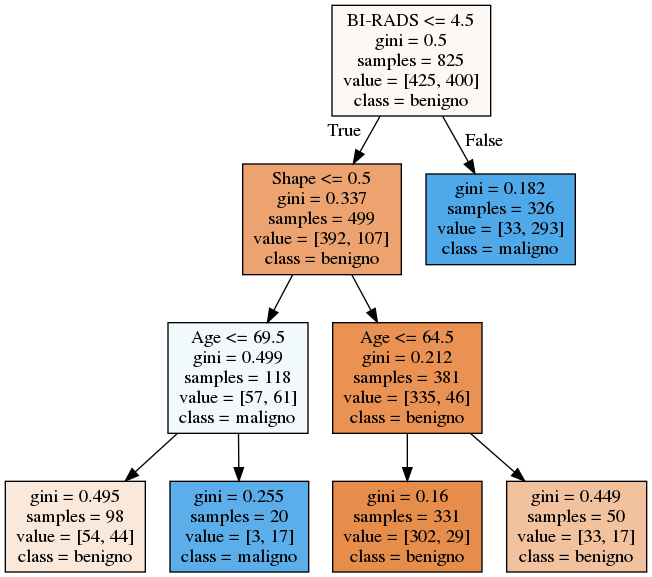
\includegraphics[width=100mm]{figures/tree_cpp}
    \caption{Árbol de Decisión obtenido con \emph{Cost Complexity
    Pruning}}
\end{figure}

que sugiere que la variable BI-RADS es la más relevante, junto con
Shape y Age, lo que no contradice al anterior criterio, aunque no
aporta información sobre Margin.

En cambio, si generamos el Árbol de Decisión simplemente limitando la
profundiad, obtenemos el siguiente árbol

\begin{figure}[H]
    \centering
    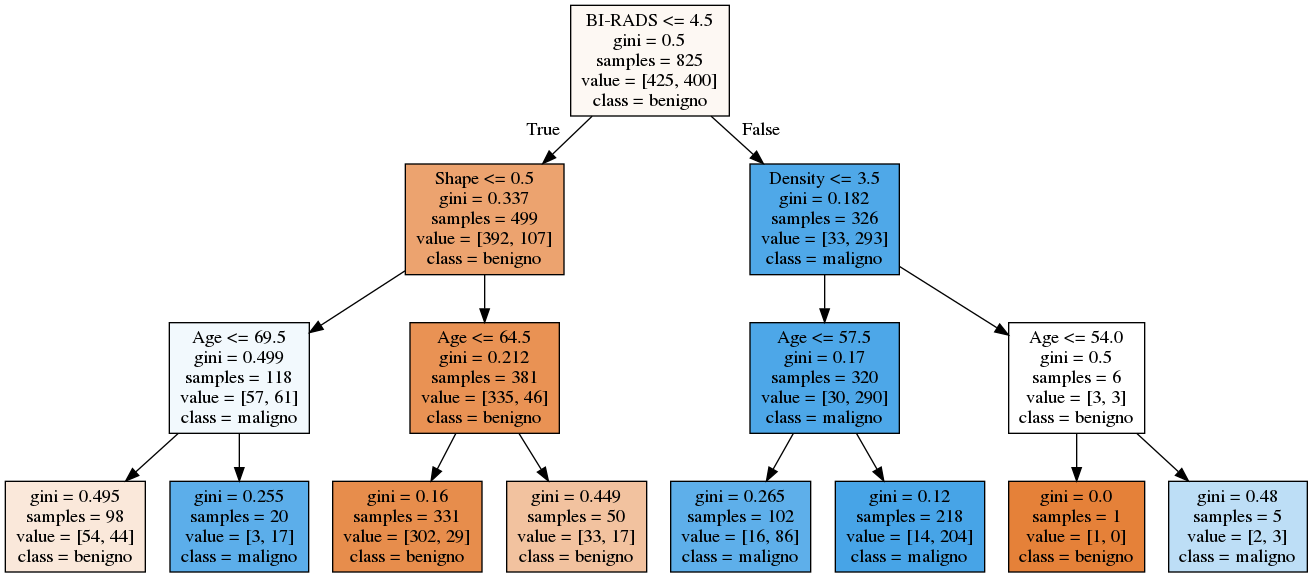
\includegraphics[width=120mm]{figures/tree_depth}
    \caption{Árbol de Decisión obtenido limitando la profundidad a 3}
  \end{figure}
  que sugiere que la variable Density puede ser relevante. Tendríamos
  que fijarnos entonces en que la reducción de impureza Gini que
  aporta es baja, luego este método puede resultar engañoso.

  En definitiva, el criterio de estimar la relevancia de las variables
  por su índice de presencia en Random Forest parece bastante más
  robusto que atender a los nodos superiores de un árbol de decisión.

  Existen otros criterios basados en Random Forest para estimar la
  relevancia de las variables, el atributo
  \href{https://scikit-learn.org/stable/modules/generated/sklearn.ensemble.RandomForestClassifier.html#sklearn.ensemble.RandomForestClassifier.feature_importances_}{\texttt{feature\_importances\_}}
  de \texttt{RandomForestClassifier} en \textit{sklearn} proporciona
  la reducción total de impureza Gini de cada variable en cada una de
  sus apariciones en los estimadores del bosque, también es un método
  bastante efectivo, pero algo más complejo de implementar e
  interpretar.

  En el archivo \texttt{RF\_feature-importance.ipynb} se encuentra el
  código utilizado para esta demostración, por si se quieren consultar
  más detalles o probar variantes.
\end{document}
